\documentclass{article}

\usepackage[utf8]{inputenc}
\usepackage[T1]{fontenc}
\usepackage{amsmath}
\usepackage{amssymb}
\usepackage{mathtools}  % for \coloneqq
\usepackage{amsthm}
\usepackage{microtype}
\usepackage[english]{babel}
\usepackage{csquotes} % for quotes in citations
\usepackage{siunitx}
\usepackage{graphicx}
\usepackage{subcaption}
\usepackage{lmodern}
\usepackage{clrscode3e}  %For Writing pseudocodes

\usepackage[backend=biber, style=alphabetic]{biblatex}

\usepackage{microtype}
\usepackage{graphicx}
\usepackage{titling}
\usepackage{titlesec}
\usepackage{environ}
\usepackage{xcolor}
\usepackage{tikz}

\definecolor{dark}{HTML}{3E454C}
\definecolor{blue}{HTML}{2185C5}
\definecolor{teal}{HTML}{7ECEFD}
\definecolor{pinkish}{HTML}{FF7F66}
\definecolor{red}{HTML}{D90000}

% Font sizes:    Calculated using 1.2^k, k=1,...,5
% 1.2
% 1.44
% 1.728
% 2.0736
% 2.48832

\newtheoremstyle{pretty}
  {\topsep}   % ABOVESPACE
  {\topsep}   % BELOWSPACE
  {\itshape}  % BODYFONT
  {0pt}       % INDENT (empty value is the same as 0pt)
  {\fontseries{b}\selectfont} % HEADFONT
  {.}         % HEADPUNCT
  {5pt plus 1pt minus 1pt} % HEADSPACE
  {}          % CUSTOM-HEAD-SPEC

\theoremstyle{pretty}



\pretitle{
    \begin{center}
    \fontsize{1.728em}{1em}\fontseries{b}\selectfont
}
\posttitle{
    \par
    \end{center}
    \vskip 0.5em
}
\preauthor{
    \begin{center}
    \fontsize{1.2em}{1.44em}\selectfont
}
\postauthor{
    \end{center}
}
\predate{
    \begin{center}
    \fontsize{1.2em}{1.44em}\selectfont
}
\postdate{
    \end{center}
}

\titleformat*{\section}{\fontsize{14.4pt}{1.728pt}\fontseries{b}\selectfont}
\titleformat*{\subsection}{\fontsize{1.2em}{1.44em}\fontseries{b}\selectfont}
\titleformat*{\subsubsection}{\fontseries{b}\selectfont}

\newcommand{\textb}[1]{{\fontseries{b}\selectfont #1}}

\NewEnviron{myBox}[1][teal!40]
{
\begin{center}
\begin{tikzpicture}
    \node [fill=#1, text width=\linewidth-1cm, align=justify, inner xsep=5mm, inner ysep=3mm] at (0, 0)
    {\BODY};
\end{tikzpicture}
\end{center}
}
\newcommand{\ds}{\mathop{ds}}
\newcommand{\dx}{\mathop{dx}}
\newcommand{\dt}{\mathop{dt}}
\newcommand{\dxdt}{\mathop{dx}\mathop{dt}}
\newcommand{\dsdt}{\mathop{ds}\mathop{dt}}

\newcommand{\R}{\mathbb{R}}
\newcommand{\placeholder}{\makebox[1ex]{\textbf{$\cdot$}}}

\renewcommand{\L}{\mathcal{L}}
\addbibresource{ref.bib}

\newtheorem{theorem}{Theorem}[section]
\newtheorem{corollary}{Corollary}[theorem]
\newtheorem{lemma}[theorem]{Lemma}


\title{TMA4183 Steel Optimization}
\author{}
\date{Spring 2020}

\begin{document}

\maketitle

\section{Introduction}
We consider the optimal control problem for the controlled cooling of steel. Our end goal is to obtain a desired temperature $\theta_d$. In order to model such a cooling process mathematically, we use linear heat equation as our state equation, given by
\begin{subequations}
   \label{eq:heat}
   \begin{align}
      \rho c_p \theta_t - \nabla \cdot (k \nabla \theta) &= 0 \quad &\text{in } \Omega \times (0,T),\label{eq:heat-in-omega} \\
      -k \frac{\partial \theta}{\partial \nu} &= u(t) (\theta - \theta_w) \quad &\text{on } \Gamma_1 \times (0,T), \label{eq:state-system-bd-1} \\
      -k \frac{\partial \theta}{\partial \nu} &= 0 \quad &\text{on } \Gamma_0 \times (0,T), \label{eq:state-system-bd-2} \\
      \theta(x, 0) &= \theta_0 &\text{in } \Omega. &
   \end{align}
\end{subequations}
Here, $u = u(t) \colon \mathbb{R} \to \mathbb{R}$ is the scalar-valued, time dependent heat transfer coefficient which acts as our unknown control, $c_p$ is the heat capacity, $k$ is thermal conductivity and $\rho$ is the density. The Neumann boundary condition in \eqref{eq:state-system-bd-1} is based on Newton's law of cooling; $\theta_w$ is the temperature of the applied coolant at the boundary. The goal is to determine a optimal $u$ such that $\theta(x, T)$ is ``as close as possible'' to some desired temperature $\theta_d$, where $T$ denotes the final time of the process. In order to model this we introduce a quadratic tracking term into the cost functional. We also require the control $u$ to be \emph{admissible}, i.e. it it possible to apply the found control $u$ in some practical manner.

More formally, we wish to minimize a cost functional of the form
\begin{subequations}
\begin{equation}\label{eq:cost-func}  % Abuse of notation?
   \min J(\theta, u) = \frac{1}{2} \int_\Omega (\theta(x, T) - \theta_d)^2 \mathop{dx} + \frac{\gamma}{2} \int_0^{T} u^2 \mathop{dt}
\end{equation}
subject to
\begin{equation}
      \theta \colon \Omega \times [0, T] \to \mathbb{R} \text{ solves \eqref{eq:heat}},
\end{equation}
and
\begin{equation}
   u \in U_{\mathrm{ad}}.
\end{equation}
\end{subequations}
We have defined $Q \coloneqq \Omega \times (0, T)$. Here $\gamma \geq 0$ is a penalizing parameter called Tikhonov regularization parameter, and the last term in $J(\theta, u)$ is a regularizing term which penalize high costs of the control.

In this report we shall first develop first-order optimality conditions for \eqref{eq:heat}, then in Section 3 we prove existence of an optimal control, then we consider two gradient-based optimisation methods; The projected Gradient and Newton's method with primal-dual active set strategy, then we consider their performance on a test problem and on a more realistic situation used in the industry, finally we discuss some further improvements to the model used here. 

\section{Main part}

In this section we will use the formal Langrange method to derive the adjoint equation and the optimality system \cite{optimalControl}. Formal in the sense that we use a lagrange multiplier $p$ without proving its existence in the derivation done here, we do that in Section \ref{proof}. The state system for our optimal control problem is given by a linear parabolic partial differential equation, in particular a heat equation

\begin{align*}
      \rho c_p \theta_t - \nabla \cdot (k \nabla \theta) &= 0 \quad &\text{in } \Omega \times (0,T) \\
      -k \frac{\partial \theta}{\partial \nu} &= u(t) (\theta - \theta_w) \quad &\text{on } \Gamma_1 \times (0,T), \\
      -k \frac{\partial \theta}{\partial \nu} &= 0 \quad &\text{on } \Gamma_0\times (0,T), \\
      \theta(x, 0) &= \theta_0 \quad &\text{in } \Omega 
\end{align*}
The domain $Q = \Omega \times (0,T)$, for the hot rolling of steel is shown in Figure \ref{fig:steel_slab}. The blue arrows represent the coolant being sprayed onto the steel slab. The boundary $\Gamma_1$ is marked, while the dashed lines represent $\Gamma_2$. 
\begin{figure}
    \centering
    % 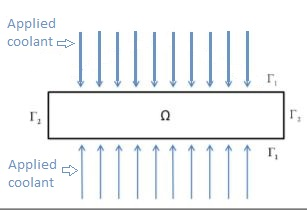
\includegraphics{figures/steel_slab_visualization.jpg}
    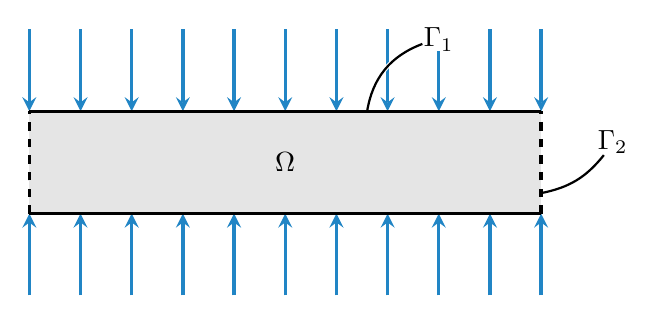
\begin{tikzpicture}[very thick, >=stealth, scale=1.3]
\draw (0, 0) -- (5, 0);
\draw (0, 1) -- (5, 1);
\draw[dashed] (0, 0) -- (0, 1);
\draw[dashed] (5, 0) -- (5, 1);
\node (domain) at (2.5, .5) {$\Omega$};
\foreach \x in {0, 0.5, ..., 5} {
    \draw[->, color=blue] (\x, -.8) -- (\x, 0);
    \draw[->, color=blue] (\x, 1.8) -- (\x, 1);
}
\node[fill=white, inner sep=0] (gamma1-1) at (4, 1.7) {$\Gamma_1$};
\node[fill=white, inner sep=0] (gamma2-1) at (5.7, 0.7) {$\Gamma_2$};
\draw[ultra thick, color=white] (gamma1-1) to [bend right=30] (3.3, 1);
\draw[thick] (gamma1-1) to [bend right=30] (3.3, 1);
\draw[thick] (gamma2-1) to [bend left=20] (5, 0.2);
\fill[black!10] (0, 0) rectangle (5, 1);
\draw (0, 0) -- (5, 0);
\draw (0, 1) -- (5, 1);
\draw[dashed] (0, 0) -- (0, 1);
\draw[dashed] (5, 0) -- (5, 1);
\node (domain) at (2.5, .5) {$\Omega$};
\end{tikzpicture}
    \caption{An illustration of our steel slab with applied cooling in blue, i.e. the control. The border $\Gamma_2$ is isolated in our modelling of the optimal control problem \eqref{eq:heat}.}
    \label{fig:steel_slab}
\end{figure}

More generally one may consider a domain $\Omega \subset \mathbb{R}^3$ which is bounded with a Lipschitz boundary, $\partial \Omega = \Gamma_1 \cup \Gamma_2$, but we will not do that here. A suitable function space for the solution of a linear parabolic PDE is 
\begin{equation}
    \label{eq:funcSpace}
    W(0,T) : = \{ \theta \in L^2(0,T;H^1(\Omega)) : \quad \frac{\partial \theta}{\partial t} \in L^2(0,T;(H^1(\Omega))^{*}) \}
\end{equation}
We endow this space with the following norm, let $u \in W(0,T)$ then 
\begin{equation*}
    \|u\|_{W(0,T)} := \bigg (\int_{0}^T\|u(t)\|^2_{H^{1}(\Omega)}\dt \bigg ) ^{\frac{1}{2}} + \bigg (\int_{0}^T\|u'(t)\|^2_{H^{1}(\Omega)^{*}}\dt \bigg ) ^{\frac{1}{2}}
\end{equation*}
This is also a Hilbert space with the inner product given by 

\begin{equation*}
    \langle u, v \rangle_{W(0,T)} := \int_{0}^T\langle u(t),v(t) \rangle _{H^{1}(\Omega)}\dt  +  \int_{0}^T \langle u'(t), v'(t) \rangle_{H^{1}(\Omega)^{*}}\dt 
\end{equation*}

We follow the notion by \cite{optimalControl} and therefore the notation $L^{p}(a,b,X)$ means the linear space of all equivalence classes of measurable vector valued functions $u:[a,b] \rightarrow X$ which have the property that
\begin{equation*}
    \int_{a}^b\|u\|_X^p \dt<\infty
\end{equation*}

We call a function vector-valued when it maps from $[a,b] \subset \mathbb{R}$ into a Banach space $X$. 

\subsection{The adjoint eqution and the gradient}
We start by finding the weak formulation for the problem defined in \eqref{eq:heat}. We multiply the equation \eqref{eq:heat-in-omega} by a test function $\psi\in W_2^{1,1}(Q)$ and integrate over the space-time cylinder $Q$. That is we multiply by a function which has weak first-order partial derivatives in space and time and second order integrability, We furthermore assume that the heat conductivity, $k$, heat capacity $c_p$ and density $\rho$ are all scalars, partial integration in space then yields 
\begin{equation}
\begin{aligned}
  0 &= \iint_Q (\theta_t - \frac{k}{\rho c_p}\Delta\theta)\psi\dxdt  \\
  &= \iint_Q \theta_t\psi\dxdt + \frac{k}{\rho c_p}\iint_Q\nabla\theta \cdot \nabla\psi\dxdt - \frac{k}{\rho c_p}\iint_{\partial Q}\partial_\nu\theta\psi\dsdt.
\end{aligned}
\end{equation}
Now after inserting for the boundary conditions defined in \eqref{eq:heat}, we end up with the following weak formulation of the state equation
\begin{equation}\label{eq:weak-form}
\begin{gathered}
  \iint_Q \theta_t\psi\dxdt + \frac{k}{\rho c_p}\iint_Q\nabla\theta \cdot \nabla\psi\dxdt + \frac{1}{\rho c_p}\iint_{\Sigma_1} u(t)(\theta - \theta_w)\psi\dsdt = 0\\
  \theta|_{t=0} = \theta_0
\end{gathered}
\end{equation}
where $\Sigma_i = \Gamma_i\times(0,T)$. We require $\theta \in W(0,T)$. Due to the isolation Neumann condition at $\Sigma_2$ only the part at $\Sigma_1$ survives. Now one can use a density argument extend this variational formulation for $\phi \in W(0,T)$ and the integrals appearing in the variational formulation are all continuous in the test function $\phi$. \bigskip

From the weak formulation of the problem, we can easily set up the Lagrangian function, by subtracting the weak formulation of the problem \eqref{eq:weak-form} from the cost functional \eqref{eq:cost-func}. The test function is replaced with a Lagrange multiplier function $p$. This gives
\begin{equation}
  \begin{aligned}\label{eq:lagrangian-raw}
  \L(\theta, u, p) = &\,J(\theta, u) - \iint_Q \theta_t p\dxdt - \frac{k}{\rho c_p}\iint_Q\nabla\theta \cdot \nabla p \dxdt \\
  &- \frac{1}{\rho c_p}\iint_{\Sigma_1} u(t)(\theta - \theta_w)p \dsdt
  \end{aligned}
\end{equation}
As we will see in Section 3, we have that our Lagrangian is a map from 
\begin{equation*}
    \L : W(0,T)\cap C(\bar{Q}) \times L^{\infty}(0,T) \times  W(0,T) \cap C(\bar{Q}) \rightarrow \mathbb{R}
\end{equation*}.

\subsubsection{Adjoint equation}
Now we derive the adjoint equation. This is done by  setting the directional derivative of the Lagrangian (with respect to the state variable) equal to zero. Assume the direction $h\in H^1(Q)$ is such that $h(x, 0) = 0$. % Antagelsen h(x, 0) = 0 popper visst ut av seg selv hvis man gjør noe på en bestemt måte i følge Dietmar.
This gives
\begin{equation}
  \begin{aligned}
  0 = \L_\theta(\theta, u, p)h = \int_\Omega (\theta(x,T) - \theta_d)h(x, T)\dx - \iint_Q h_t p\dxdt \\
  - \frac{k}{\rho c_p}\iint_Q\nabla h\nabla p \dxdt
  - \frac{1}{\rho c_p}\iint_{\Sigma_1} u(t)h p\dsdt.
  \end{aligned}
\end{equation}
Partial integration in time and in space then yields
\begin{equation} % Skip this calculation?
  \begin{aligned}
  0 = \L_\theta(\theta, u, p)h = \int_\Omega \theta(x,T) - \theta_d)h(x, T)\dx - \int_\Omega hp\Big|_0^T \dx \\
  + \iint_Q h p_t\dxdt
  + \frac{k}{\rho c_p}\iint_Q h\Delta p \dxdt \\
  - \frac{k}{\rho c_p} \iint_{\partial Q}\partial_\nu p\cdot h\dsdt
  - \frac{1}{\rho c_p}\iint_{\Sigma_1} u(t)h p\dsdt.
  \end{aligned}
\end{equation}
After some reordering of the terms we get
\begin{equation}
  \begin{aligned}
  0 = \L_\theta(\theta, u, p)h = \int_\Omega \theta(x,T) - \theta_d-p(x, T))h(x, T)\dx \\
  + \iint_Q h \left( p_t + \frac{k}{\rho c_p}\Delta p\right) \dxdt
   - \frac{k}{\rho c_p} \iint_{\Sigma_0}\partial_\nu p\cdot h\dsdt \\
   - \frac{1}{\rho c_p} \iint_{\Sigma_1}h(  k\partial_\nu p + u(t)p )\dsdt.
  \end{aligned}
\end{equation}
Now we let $h\in H_0^1(Q)$ i.e. vanishing at the boundary. Then we are only left with the second integral, which must still be equal to zero for every $h$ in the chosen function space. We then get that
\begin{equation*}
  \rho c_p p_t + k\Delta p = 0 \quad\textrm{ in } \Omega.
\end{equation*}
Letting $h\in H^1(Q)$ such that $h(x, T) = 0$ and $h|_{\Sigma_0}=0$ gives that
\begin{equation*}
  -k\frac{\partial p}{\partial\nu} = u(t)p \quad\textrm{ in } \Sigma_1.
\end{equation*}
Now we replace the last condition on $h$ from above with $h|_{\Sigma_1}=0$ and get
\begin{equation*}
  -k\frac{\partial p}{\partial\nu} = 0 \quad\textrm{ in } \Sigma_0.
\end{equation*}
We finally let $h\in H^1(Q)$, and are then left with
\begin{equation*}
  p(x, T) = \theta(x, T) - \theta_d
\end{equation*}
This constitutes the \textit{adjoint equation}, which we restate below
\begin{subequations}\label{eq:adjoint-system}
   \begin{align} % Approved by Dietmar!
      \rho c_p p_t + k\Delta p &= 0 \quad\qquad\textrm{ in } \Omega \times (0,T) \label{eq:adjoint-system-eqn} \\
      {-k}\frac{\partial p}{\partial\nu} &= u(t)p \,\,\quad\textrm{ in } \Sigma_1 \label{eq:adjoint-system-bd-1} \\
      {-k}\frac{\partial p}{\partial\nu} &= 0 \,\quad\qquad\textrm{ in } \Sigma_0 \label{eq:adjoint-system-bd-2} \\
      \rho c_p p(x, T) &= \theta(x, T) - \theta_d. \quad \textrm{ in } \Omega
   \end{align}
   \label{eq:adjoint-eqn}
\end{subequations}
This adjoint equation for the adjoint state $p$ runs backwards in time, but since the final condition i.e. $p(x,T)$ is predescribed instead of the initial condition, the problem is well-posed. If one had posed $p|_{t=0}$ instead one would have gotten an ill-posed backward parabolic equation. The driving force is end-temperature difference between the desired state and the actual temperature state of the steel slab.

\subsubsection{Gradient}
We continue with the assumption about box-constraints \eqref{eq:box_constraints}, then we can derive the variational inequality which is a first-order neccessary optimality condition to be satisfied by an optimal control $\bar{u} \in U_{ad}$. The variational inequality is given by 
\begin{equation*}
    \L_u(\bar{\theta},\bar{u},p)(u-\bar{u}) \geq 0 \text{ for } \forall u\in U_{ad}
\end{equation*}
Let $h = u - \bar{u}$, we differentiate in direction $h$, but now note that $h\in H^1(0, T)$. This gives
\begin{equation}
\begin{aligned} % Fikk hjelp av Dietmar for denne, så den skal være good.
  \L_u(\theta, u, p) h &= \gamma\int_0^T uh \dt - \frac{1}{\rho c_p} \iint\limits_{0\,\,\Gamma_1}^{\,\,\,T}(\theta - \theta_w)ph \dsdt \\
  &= \int_0^T h \left( \gamma u - \frac{1}{\rho c_p} \int_{\Gamma_1}(\theta - \theta_w)p \mathop{ds} \right) \dt.
\end{aligned}
\end{equation}
There inserting back for $h$ we have derived the variational inequality for our system, which states that
\begin{equation}
    \label{eq:variational}
    \int_0^T (u - \bar{u})(t) \left( \gamma \bar{u} - \frac{1}{\rho c_p} \int_{\Gamma_1}(\bar{\theta} - \theta_w)p \mathop{ds} \right) \dt \geq 0 \text{ for } \forall u \in U_{ad}
\end{equation}

The gradient of the reduced cost funtional $F(u) := J(y(u),u)$ can be obtained from 
\begin{equation*}
    F'(u) = \L_u(y(u),u,p(u))
\end{equation*}

The space $H^1(0,T)$ is a hilbert space. By Riesz representation theorem we can identify $H$ with $H^{*}$ for any Hilbert space $H$. Therefore by identifying using an isomorphism we find that the $u$-derivative of the lagrangian and consequently the gradient of our reduced cost functional is

\begin{equation*}
    F'(u) = \L_u(\theta,u,p) = \gamma u - \frac{1}{\rho c_p}\int_{\Gamma_1}(\theta - \theta_w)p \ds.
\end{equation*}


\subsection{Optimality System}
Now the optimality system of our control problem, \eqref{eq:heat} consists of the state equation, the adjoint equation and the variational inequality, the two latter are obtained by requiring that the $y$- and $u$-derivative of the Lagrange function do vanish. Therefore the total optimality system become
%
\begin{align*}
    \begin{cases}
     \rho c_p \theta_t - \nabla \cdot (k \nabla \theta) = 0 \quad & \text{in $\Omega$}, \\
      -k \frac{\partial \theta}{\partial \nu} = u(t) (\theta - \theta_w) &\text{on } \Gamma_1, \\
      -k \frac{\partial \theta}{\partial \nu} = 0  &\text{on } \Gamma_0, \\
      \theta(x, 0) = \theta_0 
      \end{cases}
      \end{align*}
      \begin{align*}
      \begin{cases}
       \rho c_p p_t + k\Delta p &= 0 \quad\qquad\textrm{ in } \Omega \\
      -k\frac{\partial p}{\partial\nu} &= u(t)p \,\,\quad\textrm{ in } \Sigma_1 \\
      -k\frac{\partial p}{\partial\nu} &= 0 \,\quad\qquad\textrm{ in } \Sigma_2 \\
      \rho c_p p(x, T) &= \theta(x, T) - \theta_d.
      \end{cases}
      \end{align*}
\begin{equation*}
      \gamma u - \frac{1}{\rho c_p} \int_{\Gamma_1} (\theta - \theta_w)p \ds =0
\end{equation*}

This system is a first order necessary optimality condition. That is if $\bar{u} \in U_{ad}$ is an optimal control to our optimal control problem and $\bar{\theta} = S(\bar{u})$ is the associated solution to the state system. Then there exists an adjoint state $\bar{p}$ such that the adjoint system is satisfied, and the variational inequality is satisfied. 


%Tror ikke vi trenger det under

\iffalse
Now one can restate this optimalilty system using the projection formula if one assume box-constraints. That is, if we assume
\begin{equation*}
    U_{\mathrm{ad}} := \{ u \in L^2(\Sigma_1): u_a(x,t) \leq u(x,t) \leq u_b(x,t) \text{ for a.e. } (x,t) \in \Sigma_1 \},
\end{equation*}
then a control $\bar{u} \in U_{\mathrm{ad}}$ and the associated state $\bar{\theta}$ is optimal if and only if it satisfy together with the adjoint state $p$ solving \eqref{eq:adjoint-eqn}  and $\gamma >0$ i.e. the regularisation parameter is positive that
\fi

%\begin{equation}
%    \label{eq:Proj_formula}
%    \bar{u(x,t)} = \mathbb{P}_{[u_a(x,t), u_b(x,t)]} \{\frac{1}{\gamma}\theta_w(x,t)p(x,t) \}
%\end{equation}
\section{Existence and uniquenes for the optimal control problem}\label{proof}

\subsection{Existence and uniqueness state system}
Need to consider the existence of a solution to the state equation. In order to do so we consider a more general linear parabolic partial differential equation, and derive existence for that PDE, and use that to conclude about the existence for our particular problem as well. Consider a general parabolic PDE with mixed boundary conditions

\begin{align}
    \label{eq:moreGen}
    u_t - Au + c_0 y = f \quad \text{in } Q = \Omega \times (0,T) \\
    \partial_{n_A} u + \alpha u = g \quad \text{on } \Sigma = \Gamma \times (0,T) \\
    u(.,0) = u_0(.) \quad \text{in } \Omega
\end{align}
It does not predescribe any difficulties by splitting the boundary $\Gamma$ into disjoint parts, and predescribe Neumann conditions on them separately. The functions $\alpha$, $\beta$, $f$ and $g$ all depend on $(x,t)$. Here $A$ is an elliptic differential operator of the following form
%
\begin{equation*}
    Af(x) := -\sum_{i,j}^N\frac{\partial}{\partial x_i}(a_{ij}(x)\frac{\partial}{\partial x_j}f(x)) \quad x\in \Omega
\end{equation*}
One need some requirements on the coefficents of the matrix $A=(a_{ij})$, that is one require $a_{ij} \in L^{\infty}(\Omega)$ and that they are symmetric i.e. $a_{ji}(x) = a_{ij}(x)$ for $x\in \Omega$. Moreover one also assumes that the uniform ellipticity condition is satisfied, that is $\exists M>0$ such that 
\begin{equation*}
    \label{eq:uniformEl}
    \sum_{i,j}^N a_{ij}(x)x_i x_j \geq M|x|^2 \quad \forall x \in \mathbb{R}^N \text{ for a.e. $x\in \Omega$}
\end{equation*}
Moreover from \eqref{eq:moreGen} we see that we have $\partial_{n_A}$ appearing which is the directional derivative of the conormal vector $n_{A}$ which is a vector whose component are given by $n_{A} = An$ where A is the elliptic differential operator. Then we can infer an existence and uniqueness theorem for the PDE given in \eqref{eq:moreGen}. 

\begin{theorem}[Existence and uniqueness] Assume that $\Omega \subset \mathbb{R}^n$ is a bounded Lipschitz domain with boundary $\Gamma$ and let $T>0$ denote the final time. Moreover if $c_0 \in L^{\infty}(Q)$ and $\alpha \in L^{\infty}(\Sigma)$, where $\alpha(x,t) \geq 0$ for a.e. $(x,t) \in \Sigma$, $y_0 \in L^2(\Sigma), f \in L^2(Q)$ and $g \in L^2(\Sigma)$. Then the parabolic initial-value problem \eqref{eq:moreGen} has a unique weak solution in $W_2^{1,0}(Q)\cap L^{\infty}(0,T;L^2(\Omega))$. Moreover, there is a constant C>0 which is independent of $f$, $g$ and $u_0$ such that 
\begin{equation*}
    \max_{t \in [0,T]}\|u(.,t)\|_{L^2(\Omega)} + \|u\|_{W_2^{1,0}(Q)} \leq C(\|f\|_{L^2(Q)} + \|g\|_{L^2(\Sigma)} + \|u_0\|_{L^2(\Omega)})
\end{equation*}
this holds for all $f \in L^2(Q), g \in L^2(\Sigma)$ and $u_0 \in L^2(\Omega)$
\end{theorem}

\begin{proof}
The proof is given by Tröllsch in \cite{optimalControl} under theorem 7.8. However we can give a rough sketch of the required steps in the proof. WOLOG one may assume that $c_0(x,t)\geq 0$ for a.e. $(x,t) \in Q$, since if that were not the case one could do the substitution $y(x,t) \rightarrow e^{\lambda t}\bar{y}(x,t)$. Then the resulting differential equation for $\bar{y}$ involves the term $(\lambda + c_0)\bar{y}$ instead of $c_0y$ as in the original PDE. Taking $\lambda >0$ large enough this will certainly be positive. 

Now in order to prove the existence in the theorem one need to proceed in 4 steps,
\begin{enumerate}
    \item Do a Galerkin approximation to the problem
    \item Estimate the sequence $\{y_n \}$ which is an approximation sequence for the states of the PDE
    \item Consider the convergence of the sequence of estimated controls $\{u_j^N\}_j$ and states $\{ y_n \}$
    \item Show that the limit $y_n \rightarrow y$ is indeed a weak solution to the PDE
\end{enumerate}
One use densness
To prove uniqueness one have to use an energy inequality together with the regularity of the solution.
\end{proof}


From this theorem we can conclude about existence of a solution to our particular parabolic PDE. Set $c_0 = 0$, $A = \frac{1}{\rho c_p}\nabla \cdot (k\nabla)$ , $f = 0$, then $\partial_{n_A} = \partial_n$ furthermore we set $\Gamma = \Gamma_1 \cup \Gamma_2$, to partition our boundary into to disjoint separate parts, now let $\alpha_1 = -\frac{u(t)}{k}$ and $g_1 = -\frac{u(t)\theta_w}{k}$, while one set $\alpha_2 = 0, g_2 = 0$, where $\alpha_i$ is the value of $\alpha$ on $\Sigma_i$ and similarly for $g_i$. This results in the next corollary. 

\begin{corollary}[Existence]
Suppose that $\theta_w \in L^{\infty}(\Sigma_1)$, $\theta_0 \in L^2(\bar{\Omega})$, $u \in L^{\infty}(0,T)$ and $u\geq 0$ then the initial value problem defined in \eqref{eq:heat} admits a unique solution $\theta \in H^{1,0}(Q)$ after a possible modification on a nullset, we have $\theta \in W(0,T)$. Morover this weak solution to the PDE satisfy and upper bound of the form 
\begin{equation*}
    \|\theta \|_{W(0,T)} \leq C\bigg ( \|g_1\|_{L^2(\Sigma)} + \|\theta_0\|_{L^2(\Sigma)} \bigg )
\end{equation*}
for a constant $C>0$ independent on $(g_1, \theta_0)$
\end{corollary}

Actually using theorem 5.5 in \cite{optimalControl} we get that our solution 
\begin{equation*}
    \theta \in W(0,T) \cap C (\bar{Q})
\end{equation*}
and as we will see the solution to the adjoint system satisfy have the same regularity using a time transformation. 


\subsection{Existence and uniqueness Adjoint system}
Want to prove that there exist a unique weak solution $p \in W_2^{1,0}(Q)$ to our adjoint system, and modifying $p$ on a nullset we get $p\in W(0,t)$. We consider the sightly more general parabolic initial-boundary value problem 
\begin{align*}
    -p_t -\nabla^2p +c_0p = a_Q \qquad \text{in } Q \\
    \partial_np + \alpha p = a_{\Sigma} \qquad \text{on } \Sigma \\
    p|_{t=T} = a_{\Omega} \qquad \text{in } \Omega
\end{align*}
if we assume bounded and measurable coefficent functions i.e. $c_0$ and $\alpha$, furtherore $a_Q \in L^2(Q)$, $a_{\Sigma} \in L^2(\Sigma)$ and $a_{\Omega} \in L^2(\Omega)$ then if we multiply by a test function and integrate, we can introduce a bilinear form
\begin{equation}
    \label{eq:parabolic_adj}
    A(y,v)(t) := \int_{\Omega}(\nabla y \cdot \nabla v + c_0(\cdot,t)yv) \dx + \int_{\Gamma}\alpha(\cdot,t)yv \ds
\end{equation}
Then we have a well-posedness result for this PDE

\begin{lemma}[Well-posedness]
The parabolic adjoint system given in \eqref{eq:parabolic_adj} has a unique weak solution $p \in W_2^{1,0}(Q)$ which is a solution to the variational problem 
\begin{equation*}
    \iint_Q pv_t \dxdt + \int_0^TA(p,v)(t)\dt = \int_{\Omega}a_{\Omega}v(T) \dt + \iint_Q a_Qv \dxdt + \iint_{\Sigma}a_{\Sigma}v \dsdt
\end{equation*}
this should hold $\forall v \in W_2^{1,1}(Q)$ with $v|_{t=0} = 0$. Now if we modify p on a nullset we have $p\in W(0,T)$ and $\exists$ a constant $M>0$ that does not depend on $(a_Q,a_{\Sigma}, a_{\Omega})$ such that 
\begin{equation*}
    \|p\|_{W(0,T)} \leq M \bigg (\|a_Q\|_{L^2(Q)} + \|a_{\Sigma}\|_{L^2(\Sigma)} + \|a_{\Omega}\|_{L^2(\Omega)} \bigg ).
\end{equation*}
\end{lemma}

\begin{proof}
The idea is to reduce it to a forward parabolic initial-boundary value problem, so we do a time transformation, take $\tau \in [0,T]$ and introduce 
\begin{equation*}
    \hat{p}(\tau) := p(T-\tau)
\end{equation*}
one does similarly with $\hat{v}(\tau)$. Then one have $\hat{p}(0) = p(T)$ and $\hat{p}(T) = p(0)$ similarly for $\hat{v}$. We have that $\hat{a_Q}(.,t):= a_Q(.,T-\tau)$ likewise for all the other coefficents, due to this time transform we have that
\begin{equation*}
    \iint_Qpv_t \dxdt = - \iint_Q \hat{p}\hat{v_{\tau}} \dxdt
\end{equation*}
Considering the weak formulation, it now corresponds to the forward parabolic initial-boundary value problem given by 
\begin{align*}
    \hat{p_{\tau}} - \nabla^2 \hat{p} + c_0 \hat{p} = \hat{a_Q} \qquad \text{in } Q \\
    \partial_n \hat{p} + \alpha \hat{p} = \hat{a_{\Sigma}} \qquad \text{on } \Sigma \\
    \hat{p}(0) = \hat{a_{\Omega}} \qquad \text{in } \Omega
\end{align*}
Now by the previous existence and uniqueness theorem this problem admits a unique weak solution $\hat{p}$ belonging to $W(0,T)$. Reversing the time transformation we have proven uniqueness and existence for the adjoint system
\end{proof}
Now this system is more general than ours, so we can reduce it to our case. Consider \eqref{eq:adjoint-eqn}, if we set $c_0 = 0$, $a_Q = 0$ and split up the boundary $\Sigma = \Sigma_1 \cup \Sigma_2$ where we set $\alpha_1 = \frac{u(t)}{k}$ and $\alpha_2 = 0$, $a_{\Sigma_i}=0$ for $i\in \{1,2 \}$ and finally set $a_{\Omega} = \theta|_{t=T}-\theta_d$ we have reduced to the case of the lemma, consequently we have existence and uniqueness for \eqref{eq:adjoint-eqn}.



\subsection{Existence of optimal control}
Under the required conditions for a solution to \eqref{eq:heat} we can go on to prove the existence of an optimal control $\bar{u}$. 

\begin{lemma}[WLSC]
    The cost functional given b y
    \begin{equation*}
         J(\theta, u) = \frac{1}{2} \int_\Omega (\theta(x, T) - \theta_d)^2 \mathop{dx} + \frac{\gamma}{2} \int_0^{T} u^2 \mathop{dt}
    \end{equation*}
    is weakly lower semicontinous (WLSC). 
\end{lemma}

\begin{proof}
We can reformulate the cost functional $J(\theta, u)$ in terms of norms as 
\begin{equation*}
    J(\theta, u) = \frac{1}{2}\|\theta (,T) - \theta_d \|_{L^2(\Omega)} + \frac{\gamma}{2}\|u\|_{L^2(0,T)}
\end{equation*}
Now a norm is convex by applying the triangle inequality and continuity of the norm follows by an application of the reverse triangle inequality. This thus implies that the cost functional is weakly lower semicontinous. 
\end{proof}

\begin{theorem}[Optimal Control]
If the assumptions in the previous theorem are satisfied, then there exist at least one solution to the optimal control problem 
\begin{align*}
       \min J(\theta, u) = \frac{1}{2} \int_\Omega (\theta(x, T) - \theta_d)^2 \mathop{dx} \mathop{dt} + \frac{\gamma}{2} \int_0^{T} u^2 \mathop{dt} \\
       \text{subject to} \\
       \rho c_p \theta_t - \nabla \cdot (k \nabla \theta) &= 0 \quad &\text{in } Q  \\
      -k \frac{\partial \theta}{\partial \nu} &= u(t) (\theta - \theta_w) \quad &\text{on } \Sigma_1, \\
      -k \frac{\partial \theta}{\partial \nu} &= 0 \quad &\text{on } \Sigma_0, \\
      \theta(x, 0) &= \theta_0 &
\end{align*}
\end{theorem}

\begin{proof}
We follow the same footsteps as in  \cite{DPSteel}. By the existence corollary for the parabolic PDE we know that  for any $u \in U_{ad} \text{ } \exists \text{ }\theta \in W(0,T)\cap C(\bar{Q})$. The set of admissible controls $U_{ad}$ is bounded in $L^{\infty}(0,T)$ therefore the solution $\theta$ is bounded in $W(0,T) \cap C(\bar{Q})$ thus the cost functional will be bounded. We can as a consequence assume we have a minimising sequence which we represent by the tuple $\{(\theta_k,u_k)\}_{k\in \mathbb{N}}$ such that we have 
\begin{equation*}
    \lim_{k\rightarrow \infty}J(\theta_k,u_k) = \inf_{(\theta,u)\in (W(0,T) \cap C(\bar{Q})\times U_{ad}}J(\theta,u)
\end{equation*}
where $(\theta_k,y_k) = S(u_k)$ where $S(.)$ is the solution operator which assigns the solution to the state system for a given control $u_k$.

Now $U_{ad}$ is a closed linear subspace of the Banach space $L^{\infty}(0,T)$, and is therefore itself a  Banach space, furthermore $U_{ad}$ is bounded and convex, so the sequence $\{u_k\}$ will be bounded, and there exist a weakly convergent subsequence of the controls $\{u_{k'} \} \subset \{u_k \}$ and a limit $\bar{u} \in L^{\infty}(0,T)$ such that
\begin{equation*}
    u_{k'} \rightharpoonup \bar{u} \text{ in } L^2(0,T)
\end{equation*}

Now since $U_{ad}$ is closed and convex, $U_{ad}$ is weakly closed, therefore $\bar{u} \in U_{ad}$. \bigskip

Using our existence corollary we know there exist a unique solution to the state system also with the control $\bar{u}$. Extracting a further subsequence if necessary still index by $k'$ we have that 

\begin{equation*}
    \theta_{k'} \rightharpoonup \theta \text{ weakly in } W(0,T) \text{ and strongly in } L^2(Q)
\end{equation*}
We want to show that this limit is a solution to the weak form of our state system. We use the weak from as derived in Section 2.1 but now with $\theta_{k'}$ and $u_{k'}$ instead 

Take a test function $\phi \in W(0,T)$ and integrate over our space-time cylinder $Q$ we then have 
\begin{align*}
    \rho c_p \int_0^T\int_{\Omega}\frac{\partial \theta_{k'}}{\partial t}\phi \dxdt + k \int_0^T \int_{\Omega}\nabla \theta_{k'} \cdot \nabla \phi \dxdt \\ + \int_0^T \bigg (\int_{\Gamma_1}\theta_{k'}\phi \ds \bigg )u_{k'}(t) \dt =
    \int_0^T \bigg (\int_{\Gamma_1}\theta_w\phi \ds \bigg ) u_{k'} \dt 
\end{align*}
We want to see what happens if we pass to the limit $k' \rightarrow \infty$ in the equation. All terms here are continuous in $u_{k'}$ and $\theta_{k'}$ we can therefore pass to the limit $k' \rightarrow \infty$. The solution to the state system is unique thus 
\begin{align*}
    \theta(\bar{u}) = \bar{\theta} 
\end{align*}

Now our functional $J$ is lower semicontinous by the previous lemma therefore we have  
\begin{align*}
    J(\bar{\theta}, \bar{u}) \leq \lim \inf_{k'\rightarrow \infty} J(\theta_{k'}, u_{k'})
\end{align*}
therefore the solution is optimal and hence there exist at least one optimal control $\bar{u} \in U_{ad}$. 
\end{proof}
\subsection{Real-world data for simulation}

To do our numerical simulations, we will first consider the thermal conducitivty, density and heat capacity to be constants, we divide by $\rho c_p$ in \eqref{eq:heat} to get 
\begin{equation*}
    \theta_t - \alpha \nabla \cdot (\nabla \theta) = 0 \quad \text{in $\Omega \times (0,T)$ }
\end{equation*}
Here $\alpha = \frac{k}{\rho c_p}$ is the Thermal diffusivity. To do a simulation we can set $\alpha = 3.352 mm^2/s$ to represents stainless steel, one could also simulate other materials by choosing other values of $\alpha$. To represent iron one set $\alpha_{iron} = 23 mm^2/s$. Furthermore we need the thermal conducitivity as it appears in the boundary conditions. Our choice of parameters is shown in Table \ref{tab:chosenParam}.
\begin{table}[h]
    \centering
    \caption{Parameters used for numerical simulation of the rolling of steel process.}
    \begin{tabular}{c|c}
    $\text{Parameter}$ & $\text{SI-unit}$ \\
    \hline
       $k$& $\SI{50.2}{\joule\per\metre\per\second\per\kelvin}$ \\
        $c_p$ & $\SI{460.5}{\joule\per\kilogram\per\kelvin}$ \\
        $\rho$ & $\SI{8500}{\kilogram\per\metre\cubed}$ \\
        $\theta_w$ & $\SI{20}{\celsius}$ \\
        $\theta_d$ & $\SI{700}{\celsius}$ \\
    \end{tabular}
    \label{tab:chosenParam}
\end{table}

Simulations using the parameters of Table \ref{tab:chosenParam} are shown in Figure \ref{fig:state_simulations}. These simulations were produced using a finite element method (FEM) as implemented in the Python package \verb|FEniCS| \cite{fenics}. We observe that in Figure \ref{fig:state_simulations_a} the temperature is steadily decreasing, as one would expect when continously applying a coolant to the steel. In Figure \ref{fig:state_simulations_b}, however, all of the cooling seems to happen somewhere between $t=\SI{2}{\second}$ and $t=\SI{4}{\second}$. Again, this agrees with the intuition of applying almost no coolant at the beginning or end of the cooling cycle, and maximum coolant (i.e. $u=1$) at $t=\SI{3}{\second}$. The temperatures achieved also seem to agree with values found in the literature. Thus, we conclude that the parameters we have chosen are reasonable, and that the model and the simulation of the model both perform well.
\begin{figure}
    \makebox[\linewidth]{
        \centering
    \begin{subfigure}[t]{3in}
        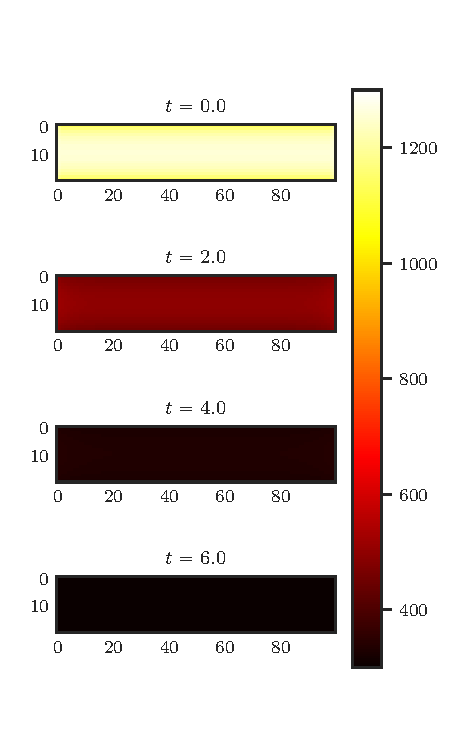
\includegraphics{figures/constant_u_state.pdf}
        \caption{Using the control $u(t)=1$.}
        \label{fig:state_simulations_a}
    \end{subfigure}
    ~
    \begin{subfigure}[t]{3in}
        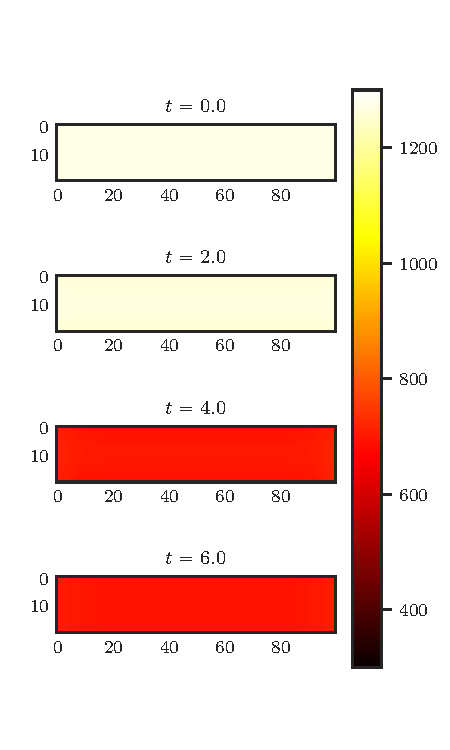
\includegraphics{figures/gaussian_u_state.pdf}
        \caption{Here, the control is $u(t) = \exp{\left(-\left(6(t-3)/10\right)^2\right)}$; a Gaussian centered around $t=3$.}
        \label{fig:state_simulations_b}
    \end{subfigure}
    }
    \caption{Simulations using the parameters given in Table \ref{tab:chosenParam}. In addition, the initial temperature of the steel was set to \SI{1300}{\celsius}. The control $u$ used is indicated in each figure caption.}
    \label{fig:state_simulations}
\end{figure}

\subsection{Improvements on the model}

A real-world simulation for the optimal cooling process of dual phase steels (DP steels) and in particular of the type Molydbenum-Magnesium in a rolling steel process can be modelled by choosing parameter with the value 
\begin{align*}
    \theta_d = \SI{680}{\celsius}
\end{align*}
One can furthermore make the model more realistic by as in \cite{DPSteelOverview} by coupling the semilinear heat equation with an ordinary differential equation that describe the evolution of steel microstructure during the cooling process. Then one consider the optimal control problem for the controlled cooling of steel profiles in order to obtain a desired temperature and a phase distribution in the steel. Such a phase transformation can in general be described by an initial value problem of the form 
\begin{align*}
    \frac{\partial f}{\partial t} = G(f,\theta ) \\
    f_{t=0} = 0
\end{align*}
Here f is a volume fraction of the new phase, G is typically a nonlinear function of its arguments. Then one can modify the heat equation to include a right-hand side term $\rho L \frac{\partial f}{\partial t}$, where $L$ is latent heat, hence the term describes realese of heat due to the phase transformation. Furthermore one have a desired phase distribution one want to obtain, denoted $f_d(x)$ one then modify the cost functional as well to obtain an approximation to the desired phase distribution. 

\section{Numerical implementation}

To solve the optimal control problem we will consider one gradient-based optimisation method. We implement the projected gradient methods, which has an infamous slow convergence rate. The implementation of Newton's method which is expected to have a superior convergence is described in Appendix \ref{Appendix}.

Both methods are gradient-based, and we need to consider the reduced optimal control problem. Let $S$ be the solution operator for our state system:  $S(u):=\theta(\placeholder ,T)$ i.e. it assigns the control to the final time solution of the state system. Then we can write our cost functional on reduced form, and our objective is then to minimize this reduced cost functional.
\begin{equation}
\label{eq:optimization_prob}
    \min_{u \in U}F(u) := J(S(u),u) = \frac{1}{2}\int_{\Omega}(S(u) - \theta_d)^2 \dx+ \frac{\gamma}{2}\int_0^Tu(t)^2\dt
\end{equation}

\iffalse
The operator S is compact. For every $u \in L^2(\Sigma)$ the state system admits a unique solution $\theta \text{ in } L^2(0,T;H^1(\Omega)) \cap C(0,T;L^2(\Omega)$, where $\theta_t \in L^2(0,T;H^1(\Omega)^{*})$. Due to the bound in Corollary 3.1.1 we have that for every $\delta \in (0,\frac{1}{2})$, there exist a constant $k_{\delta}$ such that 
\begin{equation*}
    ||S(u)||_{H^{\delta}(\Omega)} \leq k_{\delta}||u||_{L^2(\Sigma)} \text{ } \forall u \in L^2(\Sigma).
\end{equation*}
As $H^{\delta}$ embeds compactly into $L^2(\Omega)$, $S$ is indeed compact \cite{primal_dual}. 
\fi


\subsection{Solution of the State- and Adjoint equations}

The state equation and the adjoint equations were both solved numerically with the finite element method, using the finite element programming framework \verb|FEniCS| \cite{fenics} in Python.


\subsubsection{State equation}

For solving the state equation system \eqref{eq:heat} we discretise $\theta$ in time using explicit Euler:
\begin{equation*}
    \theta_t \approx \frac{\theta^{n+1} - \theta^n}{\Delta t}.
\end{equation*}
This is inserted into the equation \eqref{eq:heat-in-omega}. As $\theta^{n+1}$ is the unknown we denote it simply by $\theta$. This gives
\begin{equation*}
    \theta - \bar{\alpha}\Delta \theta = \theta^n, \quad\textrm{where}\quad \bar{\alpha} = \alpha\Delta t,
\end{equation*}
where $\alpha$ is the thermal diffusivity defined in the previous section. We now multiply with a test function $v\in H^1(\Omega)$, and integrate over the domain to get
\begin{equation*}
    \int_\Omega \theta v \dx - \bar{\alpha}\int_\Omega \Delta\theta\dx = \int_\Omega \theta^n v\dx.
\end{equation*}
For the implementation it is convenient to combine the two Neumann boundary conditions \eqref{eq:state-system-bd-1} and \eqref{eq:state-system-bd-2} into the following expression:
\begin{equation*}
    -k\frac{\partial \theta}{\partial n} = \beta(x)u(t)(\theta - \theta_w) \quad\text{where}\quad \beta(x) = \chi_{\Gamma_1},
\end{equation*}
where we have used an indicator function in the definition of $\beta$.
Partial integration then lead to the weak form
\begin{equation*}
\begin{aligned}
    \int_\Omega \theta v\dx + \bar{\alpha}\int_\Omega\nabla\theta\nabla v\dx &+ \frac{\bar{\alpha}}{k}\int_{\partial\Omega}\beta(x)u(t)\theta v\ds \\
    &= \int_\Omega\theta^n v\dx + \frac{\bar{\alpha}}{k}\int_{\partial\Omega}\beta(x)u(t)\theta_w v\ds.
\end{aligned}
\end{equation*}
The left hand side is a bilinear map and the right hand side is a linear functional, so we write
\begin{equation*}
    a_S(\theta, v) = L_S(v; \theta^n).
\end{equation*}
In the implementation we set $\theta^0$ using the initial condition given in the system \eqref{eq:heat}, and solve the equation above iteratively forward in time.

\subsubsection{Adjoint equation}

The adjoint system \eqref{eq:adjoint-system} is solved backwards in time. For the time discretization of $p$ we again use explicit Euler, so we let 
\begin{equation*}
 p_t \approx \frac{p^{n+1} - p^n}{\Delta t}.
\end{equation*}
Since the equation is solved backwards in time it is now $p^n$ that is the unknown, so we denote this by $p$ and insert it into the adjoint system \eqref{eq:adjoint-system-eqn}. We then get
\begin{equation*}
    p - \bar{\alpha}\Delta p =  p^{n+1}.
\end{equation*}
% Now multiply with a test function $v\in H^1(\Omega)$ and integrate over the spatial domain to get
% \begin{equation*}
% \int_\Omega pv\dx - \Delta t\frac{k}{\rho c_p}\int_\Omega % \Delta p v \dx = \int_\Omega p^{n+1} v \dx
% \end{equation*}
Again we combine the two Neumann boundary conditions \eqref{eq:adjoint-system-bd-1} and \eqref{eq:adjoint-system-bd-2} into one expression:
\begin{equation*}
    -k\frac{\partial p}{\partial n} = \beta(x)u(t)p,
\end{equation*}
with $\beta$ as defined above. Once more, we multiply with a test function $v\in H^1(\Omega)$ and integrate over the spatial domain. The partial integration then leads to the weak form
\begin{equation*}
    \int_\Omega pv\dx + \bar{\alpha} \int_\Omega \nabla p \nabla v \dx + \frac{\bar{\alpha}}{k}\int_{\partial\Omega} \beta(x)u(t)pv \ds  = \int_\Omega p^{n+1}v\dx.
\end{equation*}
For the \verb|FEniCS| implementation we let the left hand side and the right hand side be the bilinear and linear form respectively, and we write
\begin{equation*}
    a_A(p, v) = L_A(v; p^{n+1}).
\end{equation*}
For the implementation we initialize $p^{T/\Delta t}$ using the end time conditions in the adjoint system \eqref{eq:adjoint-system}, and then solve the system above at each time step, backwards in time.


\subsection{Projected Gradient Descent}

The idea of a descent method is to iteratively approach an optimal control. This is done through starting with some initial guess $u_0$, and then finding some \emph{descent direction} $d_k$ and an associated step size $a_k$ at a given iteration $k$, where our control will then be given by $u_{k+1} = u_{k} + a_k d_k$. One obvious requirement is thus
\begin{equation*}
    F(u_k + \alpha_kd_k) < F(u_k).
\end{equation*}
Using the Taylor expansion of $F$ around $u_k$, we get a way to choose the descent direction:
%typically one can take different means to decide this, but a descent direction can in general be chosen by 
\begin{equation*}
    d_k = \arg\min_{\|d\|_U=1} \langle \nabla F(u_k), d \rangle_U.
\end{equation*}
Gradient descent gets its name from choosing the descent direction by setting $d_k = -\nabla F(u_k)$.

Next, one need to determine how far to go in that direction. This is denoted by $\alpha_k$, called the step length, or the \textit{line search} parameter. The ideal such parameter is 
\begin{equation*}
    a_k = \arg \min_{\alpha>0} \{ F(u_k + \alpha d_k) \}.
\end{equation*}
There are different ways to choose this line search step. One require a couple of properties to be satisfied these are
\begin{align*}
    F(u_k + \alpha_kd_k) < F(u_k) \text{  } \quad\forall k \\
    F(uk + \alpha_k d_k) - F(u_k) \rightarrow 0 \text{ as } k\rightarrow \infty.
\end{align*}
We stick with Armijo rule as our line search strategy. This method consists of given a descent direction $d_k$ of F at $u_k$, choose the largest $a_k \in \{ \beta^0, \beta, \beta^2,..,\beta^m,... \}$ such that
\begin{equation}\label{eq:armijo}
    F (u_k + \alpha_kd_k) - F(u_k) \leq \mu \alpha_k \langle \nabla F(u_k),d_k \rangle_{U}
\end{equation}
where $\mu,\beta  \in (0,1)$ are chosen constant, that is we use backtracking to determine the stepsize \cite{iterativeMethods}. We set $\mu = 10^{-4}$ and $\beta = \frac{1}{2}$. More facts about Armijo rule and the convergence properties of this line search strategy is in \cite{numMethods, iterativeMethods}.

We need to ensure the computed control is within the admissible set of controls $U_{\textrm{ad}}$. In our case, we have box constraints given in \eqref{eq:box_constraints}, that is we have a lower bound $u_a$ and upper bound $u_b$ for the control variable. We use a projection onto the set of admissible controls, explaining the name \emph{projected gradient descent method}. We use a simple cut-off function, i.e. a projection given by
\begin{equation}
    \label{eq:projection}
    \mathbb{P}_{[u_a,u_b]}(v) := \max \{u_a, \min \{u_b,v \} \}
\end{equation}
If $u_a$ and $u_b$ are vectors, the equality should be read component-wise. Notation is similar to that found in \cite{Algorithms}. The projection must be implemented in every step of the gradient descent method and Armijo's rule. That is we consider the projected Armijo's rule given by 

\begin{align*}
    \text{Determine $\alpha_k \in \{1, \frac{1}{2},\frac{1}{4},.. \}$ such that }\\
    F \bigg (\mathbb{P}_{[u_a,u_b]}(u_k + \alpha_kd_k) \bigg ) - F(u_k) \leq \mu \alpha_k \langle \nabla F(u_k),d_k \rangle_{U}
\end{align*}


A pseudocode for the whole Projected Gradient Descent method is shown in Algorithm 1. We introduce two stopping criterions: one based on the minimum allowed step length, and one on the difference in the computed values of the control given by 
\begin{equation}
    \label{eq:stopping}
    \tau := \|u^{(k+1)} - u^{(k)}\|_U 
\end{equation}
This is to check that the controls converge towards a value, $U$ being the space of the controls. When $\tau$ becomes smaller than some predetermined value, abort the procedure and return the result.


\begin{codebox}
\Procname{$\proc{Algorithm 1: Projected Steepest Descent with Armijo}$}
\li Choose initial value $u^{(0)}\in U_{ad}$
\li Set tolerance $\id{tol}$ and $\alpha_{min}$
\li Solve state system to obtain $\theta^{(0)}$, with $u^{(0)}$
\li Solve adjoint system to obtain $p^{(0)}$, with $u^{(0)}$ and $p^{(0)}$
\li $k=0$
\li \While ($\tau > \id{tol}$)  \Then
\li Choose the descent Direction $d_k = -\nabla F(u^{(k)})$
\li Use the Projected Armijo rule to determine $\alpha_k$
\li \If $\alpha_k < \alpha_{min}$ \Then 
\li \textbf{Break} \End
\li Set $u^{(k+1)} = \mathbb{P}_{[u_a,u_b]}\bigg (u^{(k)} + \alpha_k d_k \bigg )$
\li Solve state system to obtain $\theta^{(k+1)}$, with $u^{(k+1)}$
\li Solve adjoint system to obtain $p^{(k+1)}$, with $u^{(k+1)}$ and $\theta^{(k+1)}$
\li Compute $\tau$
\li $k = k +1$
\end{codebox}

The gradient of our reduced cost functional is given by
%
\begin{equation*}
    \nabla F(u) =  \gamma u - \frac{1}{\rho c_p} \int_{\Gamma_1} (\theta - \theta_w)p \ds = 0
\end{equation*}
%
The projected gradient descent method is globally convergent if the reduced cost functional $F$ is Fréchet differentiable and bounded from below. As the solution to the state system $S(u) \in W(0,T) \cap C(\bar{Q})$, $F$ is indeed Fréchet differentiable. Moreover, we have that $F(u) \geq 0$ for all choices of controls $u \in U_{ad}$ by the definition of $F(u)$. Therefore, we have global convergence. However, this is a first-order descent method, and the convergence rate is typically very slow, as it solely relies on first-order gradient information. We expect to see big improvements when the control $u_k$ is far from the optimal, with diminishing improvements as we get closer and closer to $\bar{u}$. \bigskip 

This behaviour is confirmed by the results shown in figure \ref{fig:armijo}. Here, we first solved the state equation with $u(t) = 1/2$, and used the mean temperature at $t=T$ from this solution as $\theta_d$. We then ran Algorithm 1 (implemented in Python) with initial guess $u^{(0)} = 0.1$, regularisation parameter $\gamma = 1$, minimum allowable normed difference between iterations $\id{tol} = 10^{-10}$, and minimum allowable step length $\alpha_{\min} = 2^{-40}$.\footnote{The values for $\id{tol}$ and $\alpha_{\min}$ are perhaps too small, and could be increased to speed up the algorithm.} The Armijo parameter from \eqref{eq:armijo} was set to $\mu=10^{-4}$. This algorithm reached a value for the control of $0.4903$ after 2 steps, an absolute relative difference of less than 2\% with respect to the correct value of $0.5$. After 9 steps the step length became unacceptably short, and the algorithm terminated with a final value of $u=0.5038$, about 0.8\% away from the correct answer. A complete summary of the values computed by the algorithm are shown in table \ref{table:armijo}. 
\begin{figure}[pb]
    \centering
    \begin{subfigure}[b]{\textwidth}
        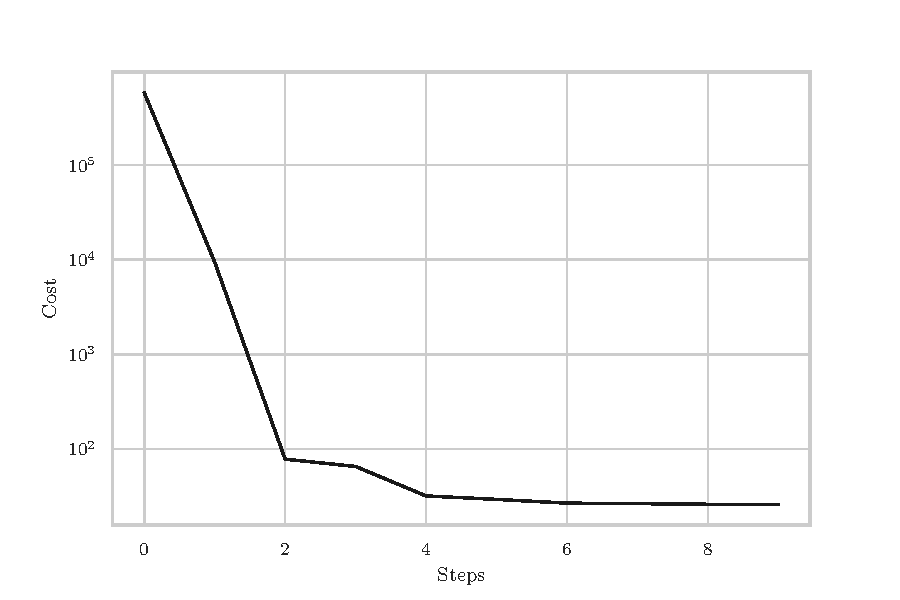
\includegraphics[width=\textwidth]{figures/cost_armijo_analytic_05.pdf}
        \caption{}
        \label{fig:armijo_cost}
    \end{subfigure}
    \begin{subfigure}[b]{\textwidth}
        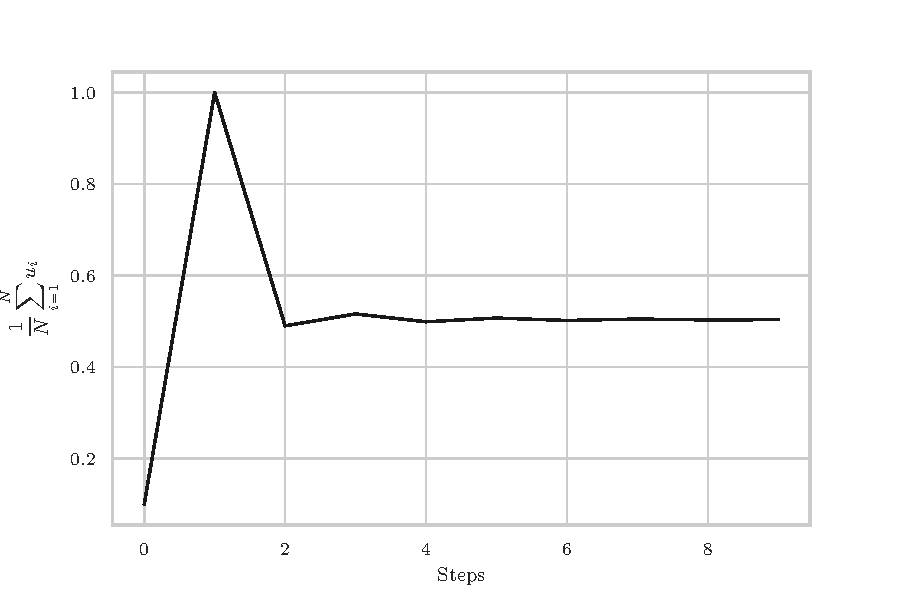
\includegraphics[width=\textwidth]{figures/U_armijo_analytic_05.pdf}
        \caption{}
        \label{fig:armijo_control}
    \end{subfigure}
    \caption{Plots showing (a) the value of the cost-function on a $\log$-scale, and (b) the associated control determined by each step of the Gradient descent algorithm with the Armijo rule. The control used to generate the desired temperature was $u(t) = 1/2$.}
    \label{fig:armijo}
\end{figure}
\begin{table}
    \centering
    \caption{Values computed by Gradient descent with the Armijo rule.}
    \label{table:armijo}
    \begin{tabular}{@{}lrSS}
         \toprule
    Step ($k$) & Step length ($\alpha$) & \multicolumn{1}{c}{Control ($u^{(k)}$)} & \multicolumn{1}{c}{$\tau = \|u^{(k-1)} - u^{(k)} \|_{\mathcal{U}}$} \\ \midrule
    0 &  & 0.1 &  \\
    1 & $2^{-13}$ & 1.0 & 6.42729 \\
    2 & $2^{-5}$ & 0.49035 & 3.63966 \\
    3 & $2^{-12}$ & 0.5162 & 0.18464 \\
    4 & $2^{-12}$ & 0.49911 & 0.12203 \\
    5 & $2^{-12}$ & 0.5073 & 0.0585 \\
    6 & $2^{-12}$ & 0.50203 & 0.03768 \\
    7 & $2^{-12}$ & 0.50511 & 0.02205 \\
    8 & $2^{-12}$ & 0.50318 & 0.01384 \\
    9 & $2^{-13}$ & 0.50376 & 0.00419 \\ \bottomrule
    \end{tabular}
\end{table}
\section{Test cases}

In the case of dual phase steel we can consider a more realistic scenario used in the industry. To do so we introduce two desired temperatures $\theta_{d_1}$ and $\theta_{d_2}$. For the optimal cooling of dual phase steel there is a phase transition in the higher temperature regime, this is modelled by the desired temperature $\theta_{d_1}$ which we want to be attained in a subset $[c_1T, c_2T]$ of $[0,T]$ with $c_2 <1$. Then we expect the optimal cooling to lead to a rapid cooling towards $\theta_{d_1}$ and stay almost constant until $t=c_2T$. Then we also expect the optimal cooling strategy to lead to a rapid cooling towards the new final desired temperature $\theta_{d_2}$. In order to model this scenario we need to introduce an extra term to the cost functional. Consequently we will get a new adjoint system, however the expression for the gradient stays the same, as the new term does not involve the control, so we can apply the Projected gradient method in Algorithm 1 almost without doing any modifications. The new cost functional is given by 
\begin{equation}
\begin{aligned}
    \label{eq:new_cost}
    J(\theta,u) : =& \frac{\alpha_1}{2}\iint_{Q}\chi_{[c_1T,c_2T]}(\theta(x,t) - \theta_{d_1}(x,t))^2 \dxdt \\
    &+ \frac{\alpha_2}{2}\int_{\Omega} (\theta(x,T) - \theta_{d_2})^2 \mathop{dx} + \frac{\gamma}{2}\int_0^T|u(t)|^2\dt
\end{aligned}
\end{equation}
Here $\chi_E$ denotes the characteristic function for the set $E$. For convenience we formulate the whole optimal control problem in this case. 
\begin{equation*}
\begin{aligned}
   \min J(\theta, u) =& \frac{\alpha_1}{2}\iint_{Q}\chi_{[c_1T,c_2T]}(\theta(x,t) - \theta_{d_1}(x,t))^2 \dxdt \\
   &+ \frac{\alpha_2}{2} \int_\Omega (\theta(x, T) - \theta_{d_2}(x))^2 \mathop{dx} + \frac{\gamma}{2} \int_0^{T} |u(t)|^2 \mathop{dt} 
\end{aligned}
\end{equation*}
subject to
\begin{align*}
       \rho c_p \theta_t - \nabla \cdot (k \nabla \theta) &= 0 \quad &\text{in } Q  \\
      -k \frac{\partial \theta}{\partial \nu} &= u(t) (\theta - \theta_w) \quad &\text{on } \Sigma_1, \\
      -k \frac{\partial \theta}{\partial \nu} &= 0 \quad &\text{on } \Sigma_0, \\
      \theta(x, 0) &= \theta_0 &
\end{align*}

We again use the formal Lagrange method to derive the adjoint system. The lagrangian takes the same form except an additional term which gives an extra contribution to the adjoint system. Taking the Frechet derivative with respect to the state of the Lagrangian we get

\begin{equation}
  \begin{aligned}
  0 = \L_\theta(\theta, u, p)h = \alpha_2 \int_\Omega (\theta(x,T) - \theta_{d_2})h(x, T)\dx - \iint_Q h_t p\dxdt \\
  - \frac{k}{\rho c_p}\iint_Q\nabla h\nabla p \dxdt
  - \frac{1}{\rho c_p}\iint_{\Sigma_1} u(t)h p\dsdt \\
  + \alpha_1 \iint_{Q}\chi_{[c_1T,c_2T]}(\theta - \theta_{d_1})h \dxdt
  \end{aligned}
\end{equation}

Then we may use partial integration, and a similar argument as used to derive the adjoint system \eqref{eq:adjoint-system} to get the adjoint system in this case. The adjoint system is given by 

\begin{subequations}
   \begin{align*} 
      \rho c_p p_t + k\Delta p + \chi_{[c_1T,c_2T]}\alpha_1(\theta - \theta_{d_1})&= 0 \quad\qquad\textrm{ in } Q  \\
      {-k}\frac{\partial p}{\partial\nu} &= u(t)p \,\,\quad\textrm{ on } \Sigma_1  \\
      {-k}\frac{\partial p}{\partial\nu} &= 0 \,\quad\qquad\textrm{ on } \Sigma_0  \\
      \rho c_p p(x, T) &= \alpha_2(\theta(x, T) - \theta_{d_2}). \quad \textrm{ in } \Omega
   \end{align*}
\end{subequations}

Now we see that we got the additional term $\chi_{[c_1T,c_2T]}\alpha_1(\theta-\theta_{d_1})$ in the PDE, thus the adjoint state $p$ depends on the temperature distribution on the interval $[c_1T,c_2T]$. As a consequence we expect to observe a non-constant control u, as mentioned we expect a rapid decay towards $\theta_{d_1}$ then a constant $u$ until $t=c_2T$ and then again a rapid decay towards $\theta_{d_2}$. Since we only consider cooling by water, we need to require $\theta_{d_1} \geq \theta_{d_2}$.



\subsection{Improvements on the model}
One can make our model more realistic as in \cite{DPSteelOverview} by coupling the semilinear heat equation with an ordinary differential equation that describe the evolution of steel microstructure during the cooling process. Then one consider the optimal control problem for the controlled cooling of steel profiles in order to obtain a desired temperature and a phase distribution in the steel, so one get an additional variable to control. Such a phase transformation in the steel microstructure can in general be described by an initial value problem of the form 
\begin{align*}
    \frac{\partial f}{\partial t} = G(f,\theta ) \\
    f_{t=0} = 0
\end{align*}
Here f is a volume fraction of the new phase, G is typically a nonlinear function of its arguments, so the phase-developement depends on temperature and the volume fraction of the phase already present. One start with zero of the given phase. 

Then one can modify the heat equation to include a right-hand side term $\rho L \frac{\partial f}{\partial t}$, where $L$ is latent heat, that is a quantity describing the release of heat due to the phase transformation. One can also vary the coolant profile, that is applied different amount of water to the different parts of the steel slab, this can be given by a function $\beta (x)$. The parabolic PDE for the temperature evolution then become 
\begin{align*}
    \rho c_p \theta_t - \nabla \cdot (k\nabla \theta) = \rho L f_t \quad \textrm{ in } Q \\
    - k \frac{\partial \theta}{\partial n} = u(t)\beta(x) \bigg (\theta - \theta_w \bigg ) \quad \textrm{ on } \Sigma_1 \\
    -k \frac{\partial \theta}{\partial n} = 0 \quad \textrm{ on } \Sigma_2 \\
    \theta(x,0) = \theta_0(x) \quad \textrm{ in } \Omega
\end{align*}

Furthermore one have a desired phase distribution one want to obtain, denoted $f_d(x)$ one then modify the cost functional as well to obtain an approximation to the desired phase distribution. That is one get a cost functional of the form 
\begin{equation*}
    J(\theta, f, u) := \frac{\alpha_1}{2}\int_{\Omega}(f(x,T)-f_d(x))^2\dx + \frac{\alpha_2}{2}\int_{\Omega}(\theta(x,T) - \theta_d(x))^2\dx + \frac{\alpha_3}{2}\int_0^Tu(t)^2 \dt
\end{equation*}

Then choosing the appropriate function $G(f,\theta)$ depends on what phase-transformation one consider, and $L$ also depends upon the chosen phase-transformation. The coolant profile $\beta(x)$ must also be chosen. Furthermore one need to choose the desired temperature profile $\theta_d(x)$ and the desired volume-fraction profile over the microstructure $f_d(x)$. All these depending on the particular application, making this a more general model than what we have been considering. 


\printbibliography
% \bibliographystyle{alphabetic}
% \bibliography{ref}  

\end{document}
